\documentclass[14pt, a2paper, portrait]{tikzposter}

\usepackage[brazil]{babel}
\usepackage[utf8]{inputenc}
\usepackage[T1]{fontenc}
\usepackage{lipsum}
 
\begin{document}

\newcommand{\bs}{\textbackslash}   
\newcommand{\cmd}[1]{{\bf \color{red}#1}}   
\tikzposterlatexaffectionproofon


\title{YOSTER ISLAND}
\author{Caio Braga Silva  Juan Victor Suman  Lucas Gomes Santana\\	    
\texttt{caiobs.99@gmail.com}
\texttt{victor.suman23@gmail.com}
\texttt{santana.lucasg@gmail.com}}

\institute{Centro Universitário Senac}

 % Set colortheme
 % (default, anil, armin, edgar, emre, hanna, james, kai, lena, manuel,
 % martin, max, nicolas, pascal, peter, philipp, richard, roman, stefanie,
 % vinay)
 
\usecolortheme{juan}

\definecolor{framecolor}{named}{black}

\settitlebodystyle{rectangular}
\setblocktitlestyle{rounded}
\setblockbodystyle{shaded}

\titleblock[left fig=logo.png, embedded]

\block[l]{Introdução}{
   O projeto foi baseado na \textit{Teoria da Evolução} de Charles Darwin levando em consideração o tema (jogo educativo). Yoster Island é baseado na linguagem \textit{C} e a biblioteca \textit{Allegro} e misturou elementos de \textit{Biologia} (conceitos da própria Teoria da Evolução como "convergência adaptiva" e "coloração de advertência") com conceitos de jogo (como RPGs) e a estética deles (em específico, de 8 bit como jogos clássicos/retrô).
}

\begin{columns}
% 1a coluna
\column{0.48}

\block[c]{Materiais e Métodos}{
	Partindo dos princípios do projeto e do objetivo, a ideia foi desenvolvida em adjunto de pesquisas teóricas (de Biologia) e conceitos de programação, tais como \textit{máquina de estados}, \textit{listas encadeadas} e outros em específico da biblioteca Allegro. O jogo em si tem dois Ambientes (dois mapas diferentes que foram dividos pelas eras, estágios de evolução do personagem) que têm inimigos definidos em certos pontos do mapa (que é dividido em diversas telas interligadas por uma lista encadeada). O jogo tem a resolução padrão de 1280 x 768 pixels. Os seres vivos foram baseados em animais reais apesar de certas liberdades estéticas e conceituais. 
	
   \begin{center}
		
\includegraphics[scale=0.48]{hqdefault.jpg} 
   \end{center} 
   
   	A parte gráfica (objetos, menus, tiles e personagens) do projeto foi desenvolvida através do \textit{Photoshop CC} levando em consideração efeitos e desenvolvimento estético de jogos antigos, tal como \textit{Pokemon Silver}. A parte sonora foi desenvolvida através do \textit{Reaper} (para a produção da música tema e efeitos sonoros) e do Audacity (para editar os efeitos sonoros). A plataforma de versionamento utilizada foi o \textit{Github}, mas para auxiliar a organização e coordenação de tarefas foi utilizado o \textit{Trello}. Para facilitar a linha de código de compilação foi feito um script em \textit{Shell script}.
}
% 2a coluna
\column{0.52}

\block[c]{Resultado}{
   \begin{center} 
   		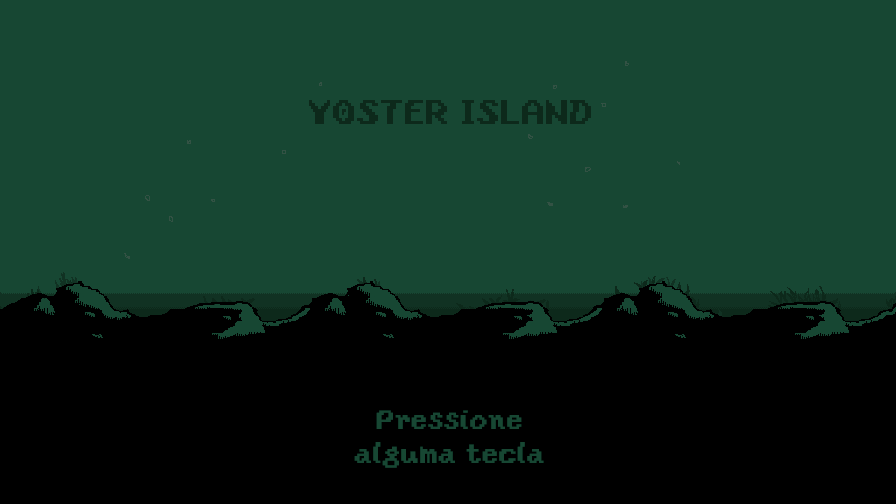
\includegraphics[scale=0.3]{../res/images/introMenu1.png} 
   		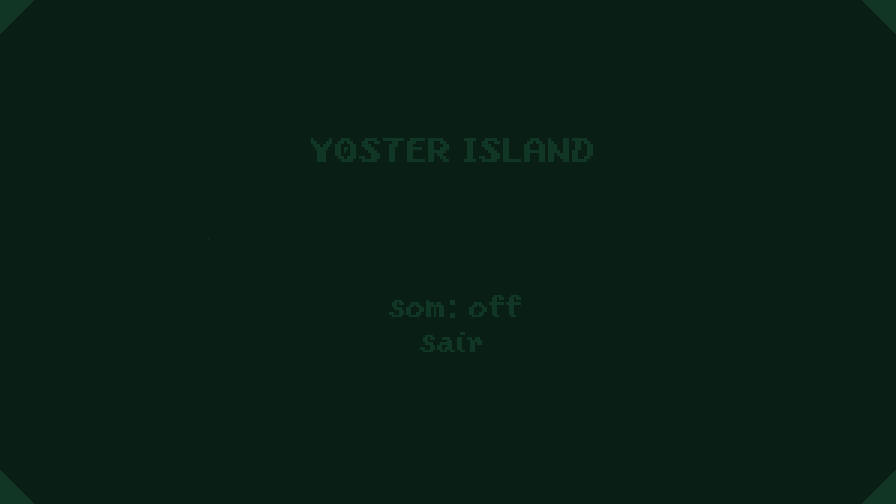
\includegraphics[scale=0.3]{../res/images/pausaPOff.png} 
   \end{center}
}

\block{Considerações Finais}{
	Infelizmente, por conta do tempo, o projeto não alcançou as expectativas iniciais (algumas irrealistas) por conta de dificuldades técnicas e a pouca experiência dos participantes com desenvolvimento de jogos eletrônicos. Ainda, é possível ver a experiência do projeto como gratificante e interessante, pois a própria experiência de organização, coordenação e desenvolvimento abriram novos horizontes por também gerar experiência com versionamento e gerar ainda mais conhecimento técnico na linguagem C e suas bibliotecas.
}

\end{columns}

\block[c,width=30cm]{Referências}{
\begingroup
   \renewcommand{\section}[2]{}
   \begin{thebibliography}{10}
	
	    \bibitem{Oetiker} OETIKER, Tobias et. al. {\sl Introdução ao {\LaTeXe}}, 2001.
		
		\bibitem{Allegro 5} ALLEGRO. {\sl Allegro 5.2.4}, liballeg.org, 2018.  

   \end{thebibliography}
\endgroup
}

\end{document}


